% Use the basic LaTeX article class, 12pt text
\documentclass[12pt]{article}

% Science uses Times font. If you don't have this installed (most LaTeX installations will be
% fine) or prefer the old Computer Modern fonts, comment out the following line
\usepackage{newtxtext,newtxmath}
% Depending on your LaTeX fonts installation, you might get better results with one or both of these:
%\usepackage{mathptmx}
%\usepackage{txfonts}

% Allow external graphics files
\usepackage{graphicx}

% Use US letter sized paper with 1 inch margins
\usepackage[letterpaper,margin=1in]{geometry}

% Double line spacing, including in captions
\linespread{1.5} % For some reason double spacing is 1.5, not 2.0!

% One space after each sentence
\frenchspacing

% Abstract formatting and spacing - no heading
\renewenvironment{abstract}
	{\quotation}
	{\endquotation}

% No date in the title section
\date{}

% Reference section heading
\renewcommand\refname{References and Notes}

% Figure and Table labels in bold
\makeatletter
\renewcommand{\fnum@figure}{\textbf{Figure \thefigure}}
\renewcommand{\fnum@table}{\textbf{Table \thetable}}
\makeatother

% Call the accompanying scicite.sty package.
% This formats citation numbers in Science style.
\usepackage{scicite}

% Provides the \url command, and fixes a crash if URLs or DOIs contain underscores
\usepackage{url}

%%%%%%%%%%%% CUSTOM COMMANDS AND PACKAGES %%%%%%%%%%%%

% Authors can define simple custom commands e.g. as shortcuts to save on typing
% Use \newcommand (not \def) to avoid overwriting existing commands.
% Keep them as simple as possible and note the warning in the text below.
% Example:
\newcommand{\pcc}{\,cm$^{-3}$}	% per cm-cubed

% Please DO NOT import additional external packages or .sty files.
% Those are unlikely to work with our conversion software and will cause problems later.
% Don't add any more \usepackage{} commands.


%%%%%%%%%%%%%%%% TITLE AND AUTHORS %%%%%%%%%%%%%%%%

% Title of the paper.
% Keep it short and understandable by any reader of Science.
% Avoid acronyms or jargon. Use sentence case.
\def\scititle{
	Personal Statement
}
% Store the title in a variable for reuse in the supplement (otherwise \maketitle deletes it)
\title{\bfseries \boldmath \scititle}

% Author and institution list.
% Institution numbers etc. should be hard-coded, do *not* use the \footnote command.
\author{
	% You can write out first names or use initials - either way is acceptable, but be consistent
	Huanan~Herman~Zhao\and
	% Someone~E.~Else$^{2}$\and
	% Additional lines of authors should be inserted using the \and command (not \\)
	% Institution list, in a slightly smaller font
	\small School of Life Sciences, Tsinghua University, Beijing \& 100084, China.\and
	% Identify at least one corresponding author, with contact email address
	\small \hspace{3em} Email: hermanzhaozzzz@gmail.com\and
	% Joint contributions can be indicated like this
	% \small$^\dagger$These authors contributed equally to this work.
}

%%%%%%%%%%%%%%%%% END OF PREAMBLE %%%%%%%%%%%%%%%%


%%%%%%%%%%%%%%%% START OF MAIN TEXT %%%%%%%%%%%%%%%
\begin{document} 

% Insert the title and author list
\maketitle

\begin{abstract} \bfseries \boldmath
    During my PhD studies, I played a pivotal role in driving advancements in genome editing technologies.
    Initially, I took the lead in developing and screening M2-CBE, 
    a refined variant of the nuclear cytosine base editor.
    This innovation significantly diminishes off-target effects on both the genome and transcriptome, 
    while upholding high on-target efficiency.
    Subsequently, I helmed a project dedicated to evaluating and improving DdCBE$_{wt}$, 
    a mitochondrial cytosine base editor. 
    Our work uncovered nuclear off-target effects induced by DdCBE$_{wt}$ and elucidated the relationship between DdCBE and CTCF.
    We alse revealed heavier off-target effects induced by enhanced DdCBE$_{DddA6/DddA11}$.
    Ultimately, we crafted strategies to effectively mitigate these off-target effects.
    More recently, I harnessed my bioinformatics expertise to independently design a sequence and structure 
    searching pipeline for discovering novel CRISPR-Cas13 candidate systems from 10Tb self-colleted genomic and metagenomic data. 
    This endeavor resulted in the experimental validation of four picked Cas13 candidates, with three confirmed as active.
    With five years of rich experience in gene editing research, 
    I have accumulated extensive knowledge of the pertinent literature and am eagerly anticipating the opportunity 
    to delve into innovative DNA/RNA editing tools and animal applications within this thrilling field.
\end{abstract}



% The first paragraph of any Science paper does NOT have a heading
% Nor is it indented
\noindent
I am about to obtain my Ph.D. degree from Tsinghua University.
My research endeavors have centered around advancing genome editing, 
specifically focusing on the safety assessment, optimization, 
and innovation of cytosine base editors (CBEs), mitochondrial cytosine base editors (DdCBEs).
The most recent year, my independent leadership work is dedicated to the discovery of novel CRISPR-Cas systems. 
This personal statement outlines my significant contributions and insights gained through these works.  

\subsection*{Unbiased detection and validation for the off-target sites of CBEs}

CBEs have the potential to correct human pathogenic point mutations\cite{komor2016programmable}. 
However, the current methods for detecting CBEs in the editome are limited. 
My initial involvement in Dr. Yi's laboratory was in the Detect-seq research project. 
This project was aimed at identifying and characterizing off-target sites in CBEs. 
The Detect-seq method, reported by our laboratory in 2021, 
utilizes the characteristic of CBEs producing deoxyuridine (dU) as an intermediate during targeted editing~\cite{lei2021detect}. 
By biotinylating and enriching the dU, and replacing adjacent cytosines with d5fC, 
Detect-seq enhances the sensitivity of detecting off-target edits (Fig.~\ref{fig:CBE_Detect_seq}a)\cite{lei2021detect}. 
This method, combined with bioinformatics analysis, 
provides high sensitivity and specificity (lower false positive rates) while eliminating interference from endogenous dU  (Fig.~\ref{fig:CBE_Detect_seq}b-d)\cite{lei2021detect,lei2022mitochondrial,lei2023detect}.  
My primary contribution was in the bioinformatics analysis and visualization of the targeted deep sequencing data, 
marking my first research achievement.  



Using Detect-seq, we identified tens to hundreds of off-target sites for BE4max in various human cell lines (Fig.~\ref{fig:CBE_Detect_seq}b).
These included classic Cas9-independent and Cas9-dependent edits, 
as well as two novel types of off-target edits: out-of-protospacer edits and target-strand edits. 
All these edits were confirmed by targeted deep sequencing (Fig.~\ref{fig:CBE_Detect_seq}d)\cite{lei2021detect}. 


  
\subsection*{Safety Assessment and Optimization of CBE variants}
Based on the findings in the previous section,
refining CBEs to minimize genomic and transcriptomic off-target effects is crucial for clinical applications. 
Blindly applying CBEs in gene therapy may cause unpredictable mutations, disrupting cellular functions and 
potentially inducing cancer ~\cite{lei2021detect,rao2023characterizing}.

My second project, which was based on my independently led and data-driven approach,
involved collaboration with a wet-lab co-worker and was focused 
on the development and characterization of the M2-CBE mutant.

  
Through rational design and mutagenesis of the rAPOBEC1 deaminase, 
we developed M2-CBE, which significantly reduced off-target editing while maintaining on-target efficiency. 
Utilizing Detect-seq (Fig.~\ref{fig:CBE_Detect_seq}a), targeted deep sequencing, and RNA-seq, 
we systematically evaluated the off-target editing of BE4max, 33A-CBE, YE1-CBE, and M2-CBE in both genome and transcriptome.
and RNA-seq, we comprehensively assessed M2-CBE's safety, 
outperforming other variants like YE1-CBE and 33A-CBE\cite{doman2020evaluation}. 
M2-CBE demonstrated precise single-base editing and reduced novel off-target types, 
advancing CBE technology's clinical potential (Fig.~\ref{fig:CBE_variants_Detect_seq}) (unpublished work).




\subsection*{Safety Assessment and Mechanistic Insights into DdCBEs}
Base editing of the mitochondrial genome (mtDNA) is a technical challenge urgently needing resolution 
in the field of gene editing before 2020. 
Novel genome editing tools such as CRISPR-Cas, Base Editor (BE), and Primer Editor (PE) rely on 
sgRNA for targeting functionality and are unable to effectively edit the mitochondrial genome.
Techniques that depend on mtZFNs, mitoTALENs, and other approaches to target and introduce 
double-strand breaks (DSBs) into the circular double-stranded DNA of the mitochondrial genome can reduce the copy number 
of mutated mitochondrial genomes, thereby decreasing the heteroplasmy level to a non-pathogenic degree within cells \cite{mok2020bacterial}. 
However, these methods also cause an overall reduction in the copy number of mitochondrial genomes within cells, 
posing additional risks and failing to fully address the issue of mitochondrial genome editing \cite{mok2020bacterial}. 
In 2020, the DdCBE, a cytosine base editor for the mitochondrial genome, was proposed. 
This tool utilizes a pair of transcription activator-like effector (TALE) proteins for targeting, 
and under the guidance of their respective tandem mitochondrial targeting signals (MTS), 
it can deliver the two halves of the novel double-stranded DNA cytosine deaminase DddA$_{tox}$, 
split by the tool, into the mitochondrial membrane. 
This allows for programmable colocalization of the two DddA$_{tox}$ halves at specified positions 
in mtDNA without opening the mtDNA double strand, thereby restoring DddA$_{tox}$ activity and introducing 
specific cytosine deamination reactions to ultimately achieve mtDNA C→T base editing \cite{mok2020bacterial}. 
DdCBE has truly enabled precise targeted editing of the mitochondrial genome, 
and this tool has quickly found applications in various systems \cite{wei2022human, chen2022ddcbe, kang2021chloroplast, guo2022ddcbe}. 
Mok et al. reported varying degrees of off-target editing by DdCBEs in mtDNA and, 
based on the analysis of DdCBE-transfected nuclear pseudogenes, claimed no off-target effects in nuclear DNA (nDNA). 
Although DdCBE represents a promising approach for treating mitochondrial diseases, 
a fair and comprehensive analysis of its off-target effects is still lacking.

Based on the history of research on mtZFNs, 
a reasonable inference regarding potential safety hazards is 
whether MTS-mediated delivery can ensure that all DdCBEs are localized in mitochondria, 
rather than partially leaking into the nucleus, thereby causing potential off-target editing \cite{gammage2014mitochondrially}. 
Therefore, it is crucial to assess the off-target effects on the nuclear genome and evaluate 
the safety of the DdCBE tool itself in samples where DdCBE has been successfully used for 
mitochondrial base editing. 
Since the base-editing mechanism of DdCBE also involves cytosine deaminase catalyzing 
the deamination of deoxycytosine in DNA to form deoxyuracil (dU), 
theoretically, Detect-seq technology can be employed to assess the off-target impact 
of DdCBE on the nuclear genome during normal mitochondrial genome base editing \cite{lei2022mitochondrial}.

I and co-workers used various omics technologies,
including Detect-seq, targeted deep sequencing, ATAC-seq, ChIP-seq, Hi-C, 
and biochemical experimental methods, to jointly complete the safety assessment of wild-type DdCBE \cite{lei2022mitochondrial}, 
the discovery and optimization of off-target mechanisms \cite{lei2022mitochondrial}, 
the safety assessment of improved DdCBE (DdCBE$_{DddA6/DddA11}$) (unpublished work), 
and the investigation of DdCBE's effects on three-dimensional 
genome structure and cell gene regulation-related functions (unpublished work).

Using omics technologies,
we found DdCBE$_{wt}$ (Fig.~\ref{fig:DdCBE_offs}b,c) 
and DdCBE$_{DddA6/DddA11}$ (unpublished work) caused substantial nuclear off-target edits (Fig.~\ref{fig:DdCBE_offs}a), 
categorized as TAS-dependent and TAS-independent  \cite{lei2022mitochondrial}. 
TAS-dependent off-target editing relies on the unilateral TALE sequence in DdCBE, 
indicating that a unilateral TALE array is sufficient to guide complete DddA$_{tox}$ to produce off-target editing, 
which contradicts the original design intent of DdCBE. 
TAS-independent off-target editing, on the other hand, does not depend on the TALE sequence. 
These sites are shared among different DdCBEs and have a preference for proximity to CTCF binding sites, 
suggesting a potential association with the three-dimensional structure of the cellular genome.

We then unexpectedly discovers a potential molecular interaction between DdCBE and CTCF 
via sequence analysis (Fig.~\ref{fig:DdCBE_offs}d), 
which is experimentally validated. 
As a key protein maintaining the three-dimensional structure of the cellular genome, 
perturbations at CTCF binding sites can have profound effects on gene expression regulation. 
The interaction between DdCBE and CTCF may explain 
the non-randomness of TAS-independent off-target editing and its enrichment at TAD boundaries. 
This finding not only broadens our understanding of the off-target mechanisms of DdCBE 
but also provides new ideas for subsequent optimization of DdCBE.

Given the extensive off-target editing in the nuclear genome caused by DdCBE, 
this study designs and validates multiple optimization strategies, 
including the introduction of nuclear export signals (NES), nuclear-localized DddI$_A$ inhibitors, 
and point mutations in DddA$_{tox}$. 
These optimization strategies significantly reduce off-target editing in the 
nuclear genome while maintaining the editing efficiency of DdCBE in the mitochondrial genome (Fig.~\ref{fig:DdCBE_offs}e). 
These achievements not only enhance the safety of DdCBE but also provide valuable references 
for the optimization of other genome editing tools.

  

\subsection*{Discovery of Novel CRISPR-Cas13 Systems}

Type VI CRISPR-Cas systems are known for their unique RNA-guided RNA cleavage activity. 
The objective of this project was to develop a bioinformatics pipeline to discover 
uncharacterized Cas13 proteins with potential biotechnological applications. 
The study utilized both public databases, such as the JGI Integrated Microbial Genomes (IMG) database and NCBI BLASTn database, 
as well as self-assembled metagenomes from \textbf{bovine rumen sequencing data}.

The mining process involved several steps, including contig analysis, CRISPR array search, 
and candidate Cas protein search within a 20kb range of CRISPR arrays. 
Candidate proteins containing HEPN motifs were selected and then clustered based on sequence similarity using MMseqs2. 
To ensure the novelty of the candidates, they were filtered against known Cas13 proteins, 
the NCBI's Non-Redundant database, the Patseq database, and manually curated literature-reported Cas13 databases. 
Proteins with more than 90\% sequence identity to known Cas13 proteins, 
those with only one HEPN motif, and duplicates were removed.

The results showed that most candidates were approximately 1100 amino acids in length and clustered 
with known Cas13 families. 
\textbf{Six out of ten candidates were derived from the self-assembled bovine rumen metagenome data}, 
highlighting the potential of metagenomic approaches in novel Cas13 discovery. 
The candidates shared around 50\% amino acid identity with their closest known Cas13 counterparts (Fig.~\ref{fig:Cas13_identity}), 
with some exceptions, and most showed high structural similarity to their known counterparts. 
CRISPR array analysis revealed that most arrays had spacer and direct repeat lengths of 30 nt and 36 nt, 
respectively, and formed stable stem-loop structures.

By expanding data sources, applying structural searching strategy (Foldseek/Dali), 
and analyzing the structure distance of the candidates (Fig.~\ref{fig:Cas13_structure_tree}), 
the study aims to explore the possibility of identifying novel RNA-guided nucleases with HEPN domains 
beyond Cas13 and study the evolutionary trajectory of the Type VI CRISPR-Cas system.

In conclusion, my study successfully identified abundant of uncharacterized Cas13 candidates.
This endeavor resulted in the experimental validation of 4 picked Cas13 candidates, with 3 confirmed as active (75\% successful rate). 

Recently, a team from Prof. Jennifer Doudna's lab published a similar and more in-depth study in \textbf{\textit{Science}}.
Although my work has not been published yet, this scientific result proves the value of my research
and provides a platform for further research in this field.

\subsection*{Insights and Future Directions}

My research not only advances the field of genome editing by enhancing the safety and efficacy of existing tools but also paves the way for the discovery of novel CRISPR systems with unique properties. The safety assessment and optimization of CBEs and DdCBEs provide critical insights into the design of future gene editors, emphasizing the importance of rigorous validation and innovation.

With five years of doctoral training in \textbf{bioinformatics and genome editing},
and an additional five years of undergraduate \textbf{education in veterinary medicine}, 
I am eager to integrate my advanced research skills with my foundational knowledge to explore innovative applications of gene editing. 
Specifically, I am passionate about leveraging these techniques in areas such as animal breeding, 
genetic modification, and xenotransplantation. 
\textbf{\textit{My primary goal for the next decade is to discover novel gene editing tools and implement them in live animal studies}}.

A toast to our field of research!

\hfill Herman,

\hfill \today

%%%%%%%%%%%%%%%% MAIN TEXT FIGURES %%%%%%%%%%%%%%%
\clearpage
\begin{figure}[htb]
	\centering
	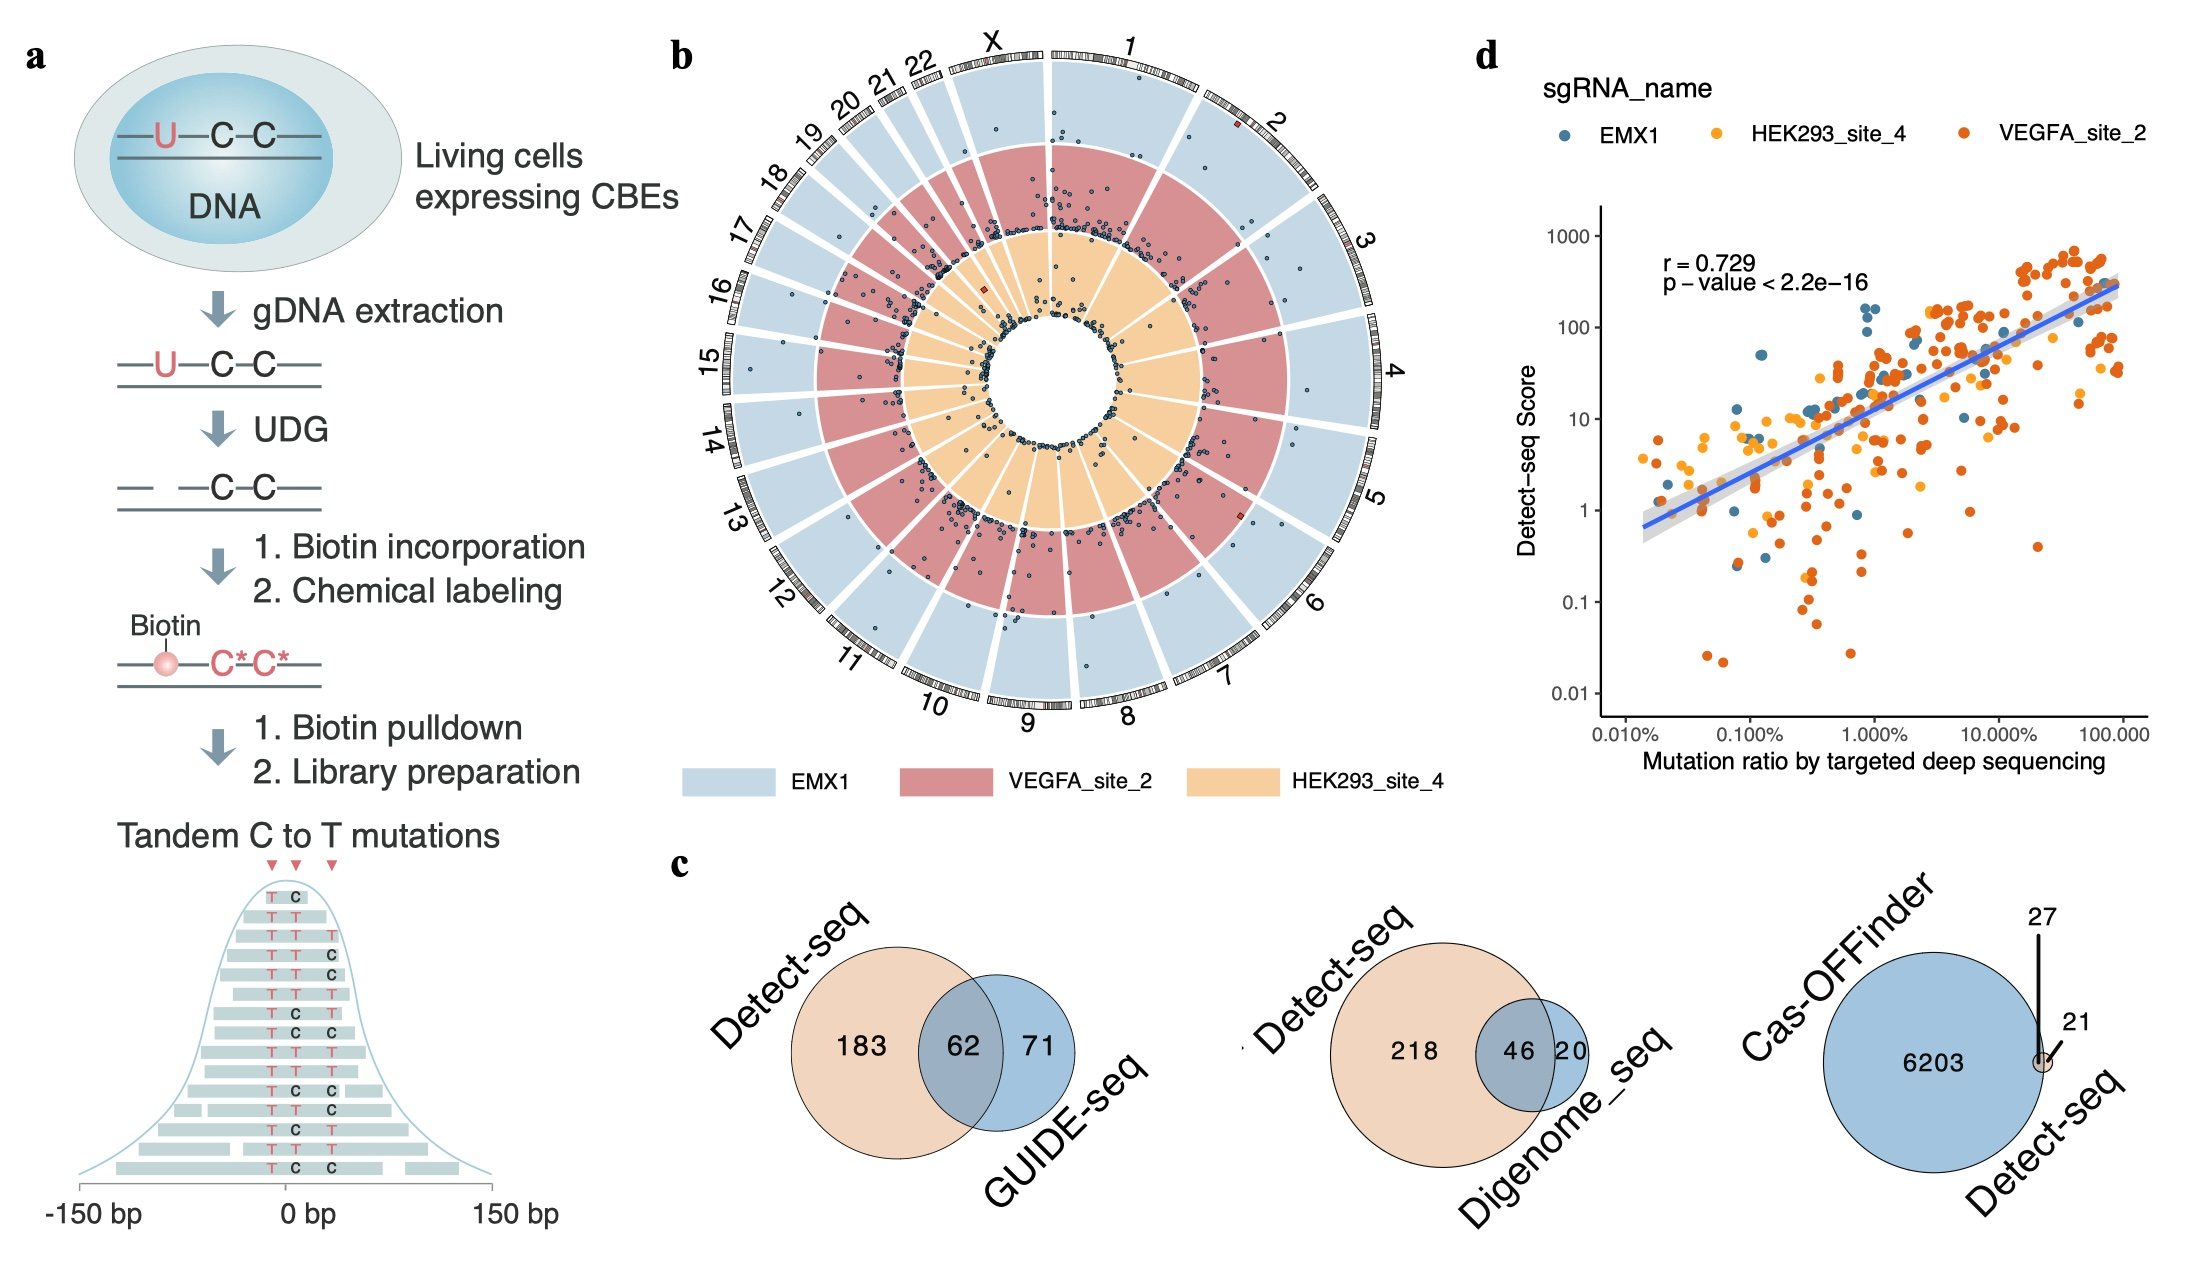
\includegraphics[width=0.9\textwidth]{figs/CBE_Detect_seq.jpg} 
	\caption{\textbf{Comparisons of Detect-seq with other methods for off-target identification.}
    \textbf{a}, Workflow of Detect-seq. 
    \textbf{b}, Genome-wide distribution of typical Cas-dependent off-target sites reported by Detect-seq.
    \textbf{c}, Venn diagrams of off-target sites identified by Detect-seq and three pre-existing methods for the HEK293\_site\_4 sgRNA.
    \textbf{d}, Log scale plot comparing the Detect-seq signals against editing ratios obtained by targeted deep sequencing.
    Adopt from \cite{lei2021detect}}
	\label{fig:CBE_Detect_seq}
\end{figure}

\begin{figure}[htb]
	\centering
	\includegraphics[width=0.7\textwidth]{figs/CBE_variants_Detect_seq.pdf} 
	\caption{\textbf{Off-target editing of BE4max, 33A-CBE, YE1-CBE, and M2-CBE in the genome reported by Detect-seq}.}
	\label{fig:CBE_variants_Detect_seq}
\end{figure}

\begin{figure}[htb]
	\centering
	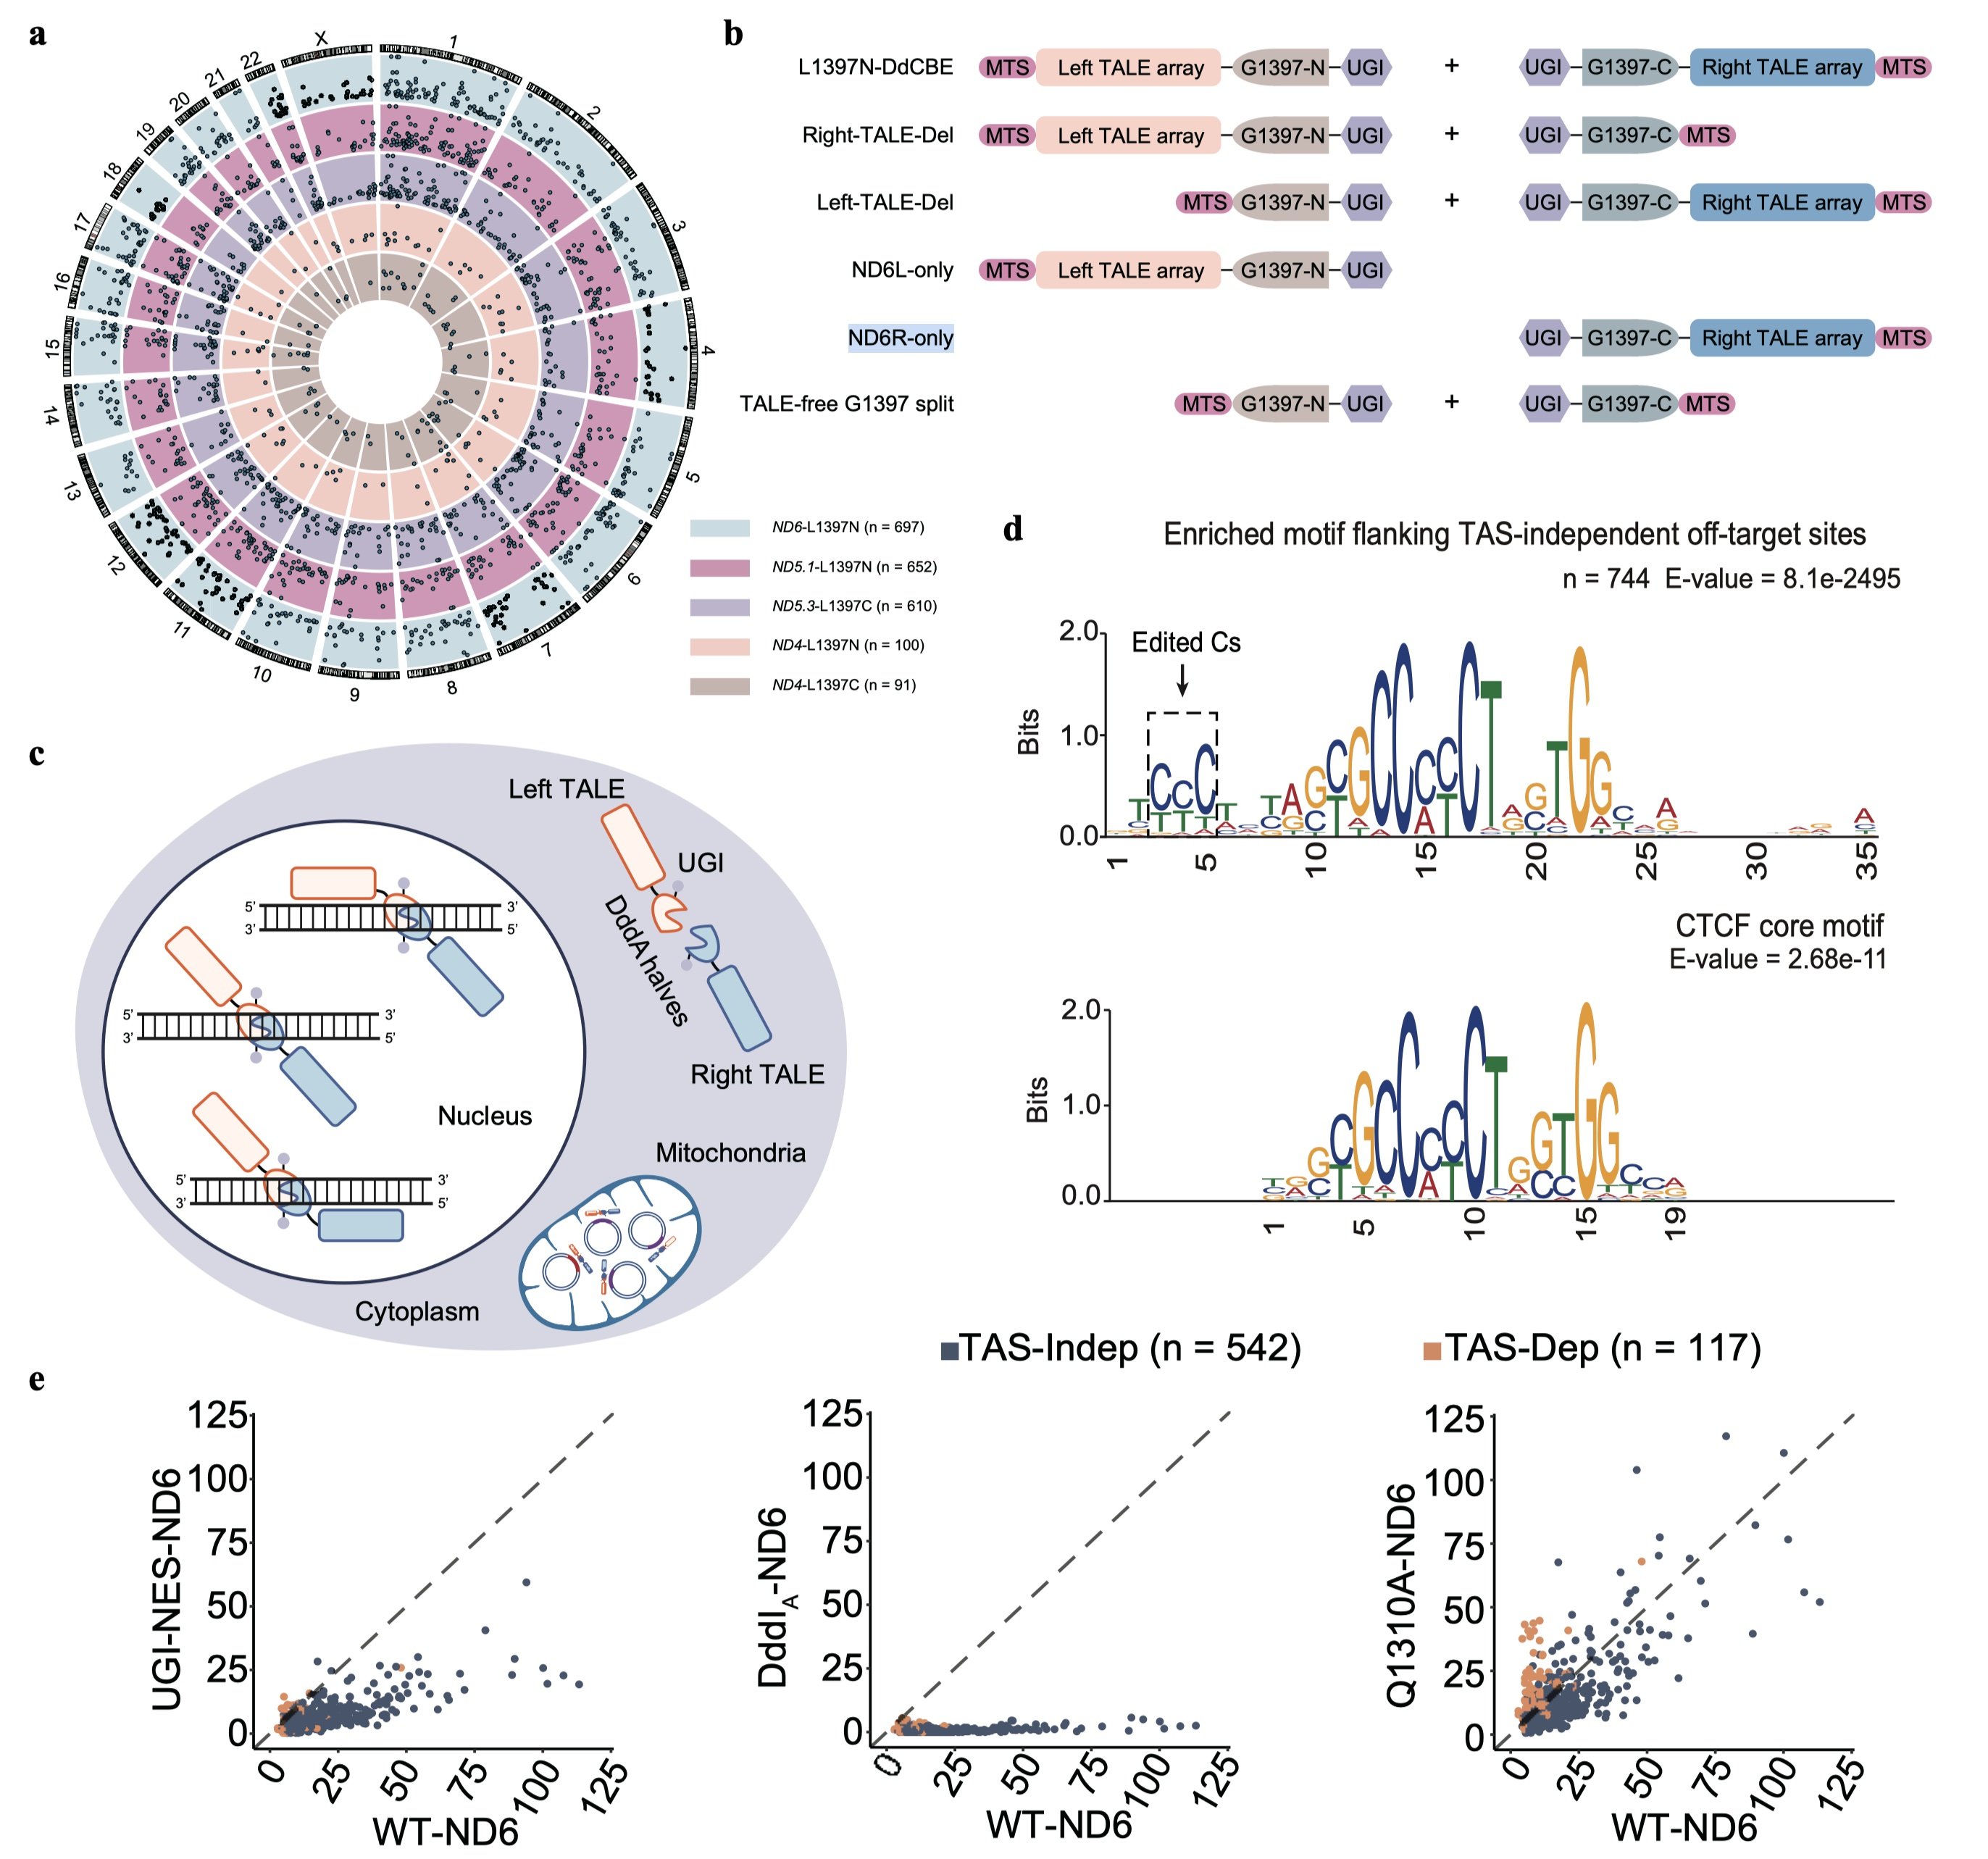
\includegraphics[width=1\textwidth]{figs/DdCBE_offs.jpg} 
	\caption{\textbf{Nuclear off-target edits induced by DdCBE$_{wt}$ and the optimization strategies to reduce off-target activity}.
    \textbf{a}, Genome-wide distribution of nuclear off-target sites reported by DdCBE$_{wt}$.
    \textbf{b}, DdCBE delete constructs.
    \textbf{c}, Scheme illustrating the off-target editing mechanisms.
    \textbf{d}, The consensus sequence downstream of the DdCBE$_{wt}$ off-target editing sites (Cs).
    \textbf{e}, The optimized DdCBE$_{wt}$ off-target sites and their strengths.}
	\label{fig:DdCBE_offs}
\end{figure}

\begin{figure}[htb]
	\centering
	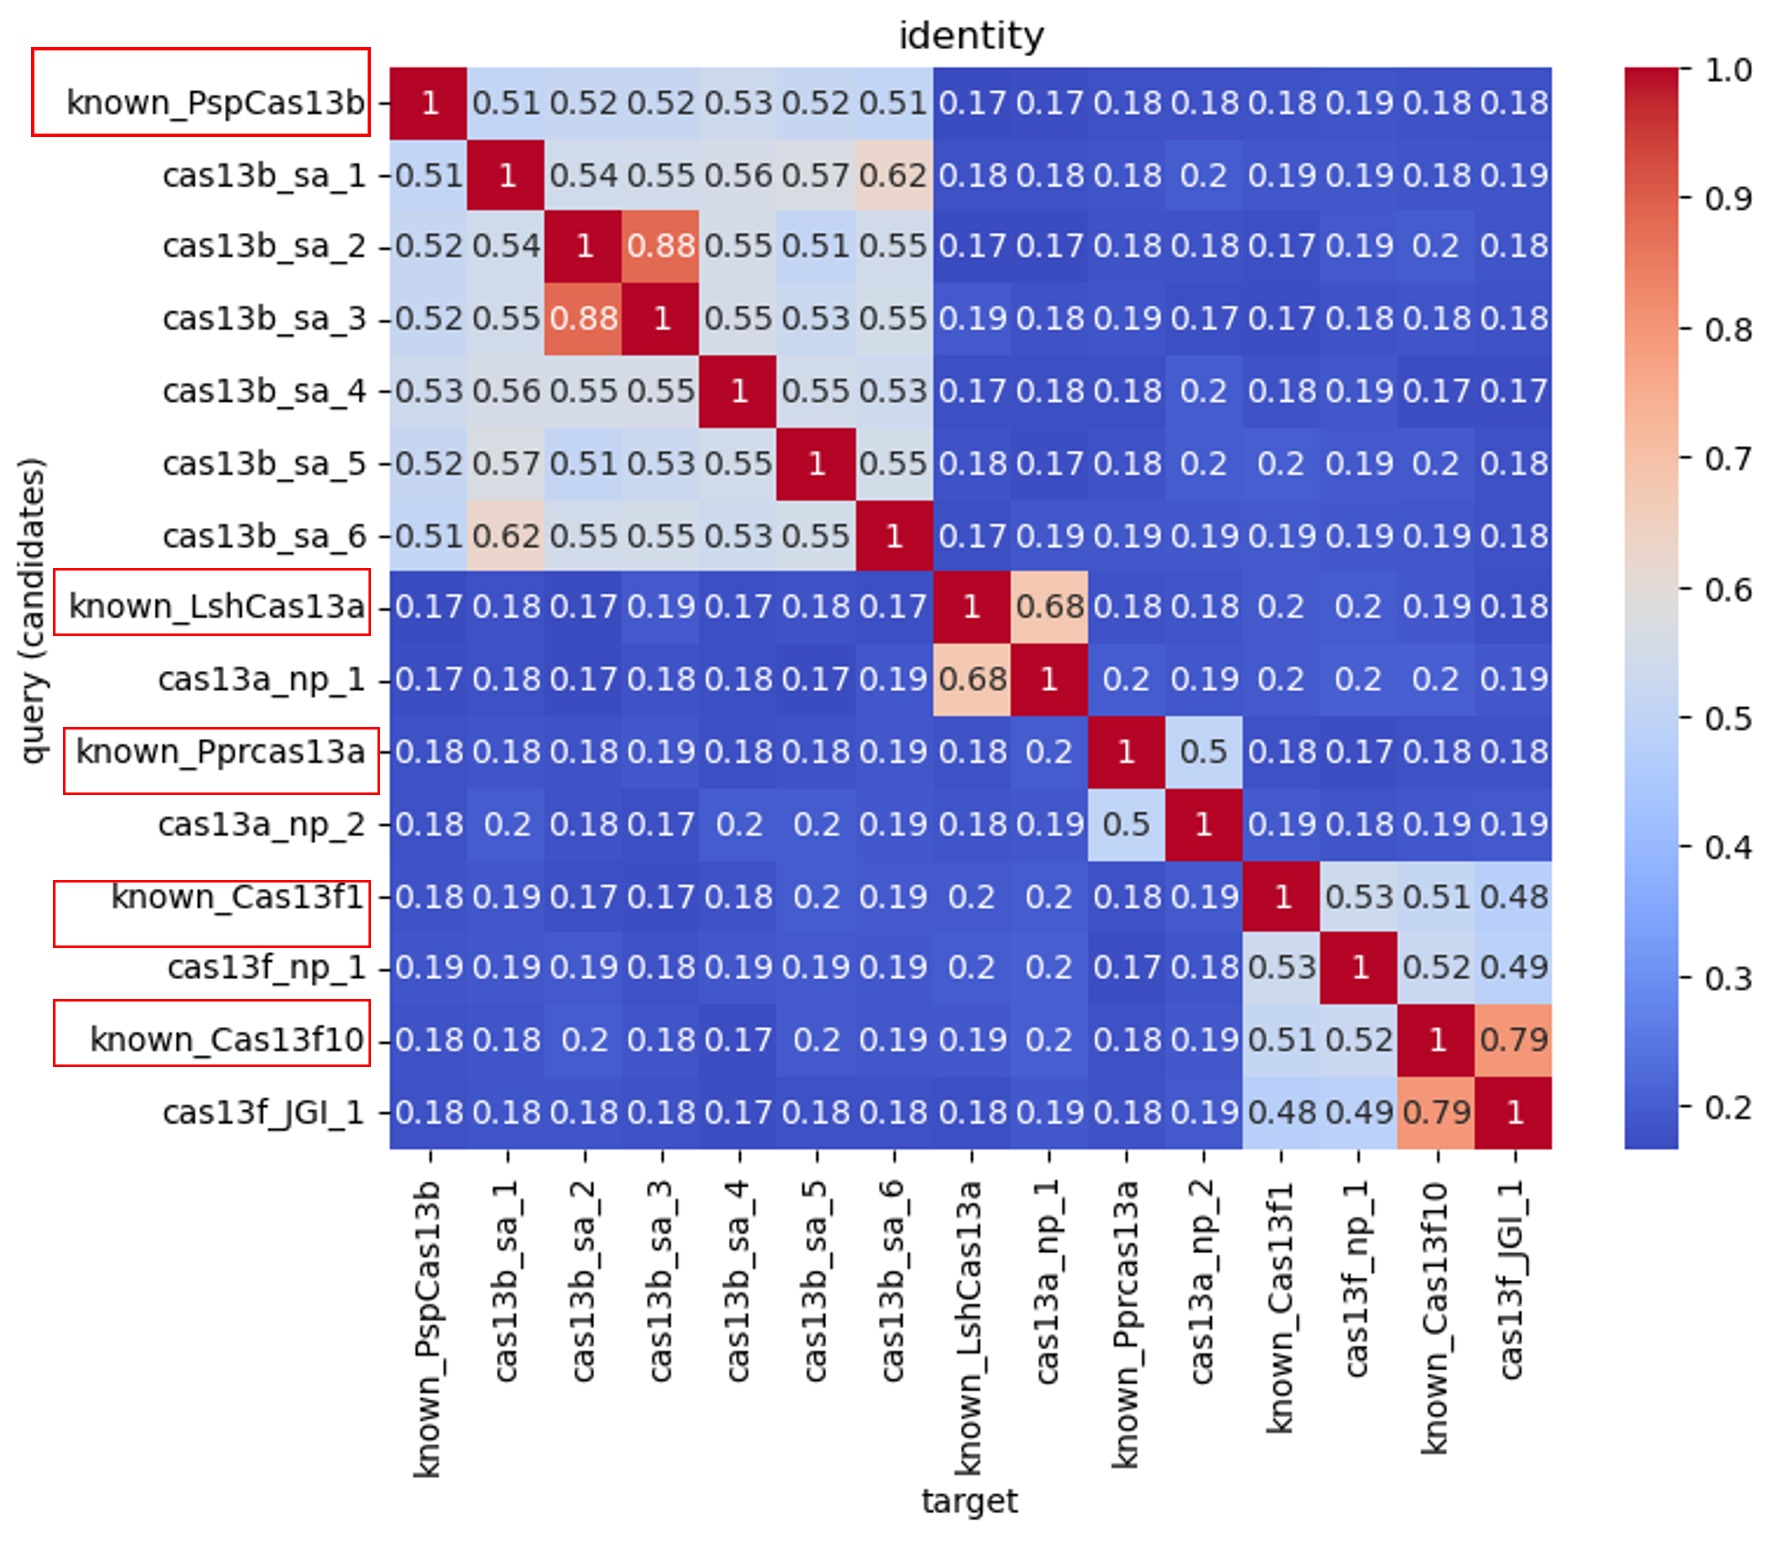
\includegraphics[width=1\textwidth]{figs/Cas13_identity.jpg} 
	\caption{\textbf{Sequence identity between new Cas13 candidates and known Cas13s}.}
	\label{fig:Cas13_identity}
\end{figure}

\begin{figure}[htb]
	\centering
	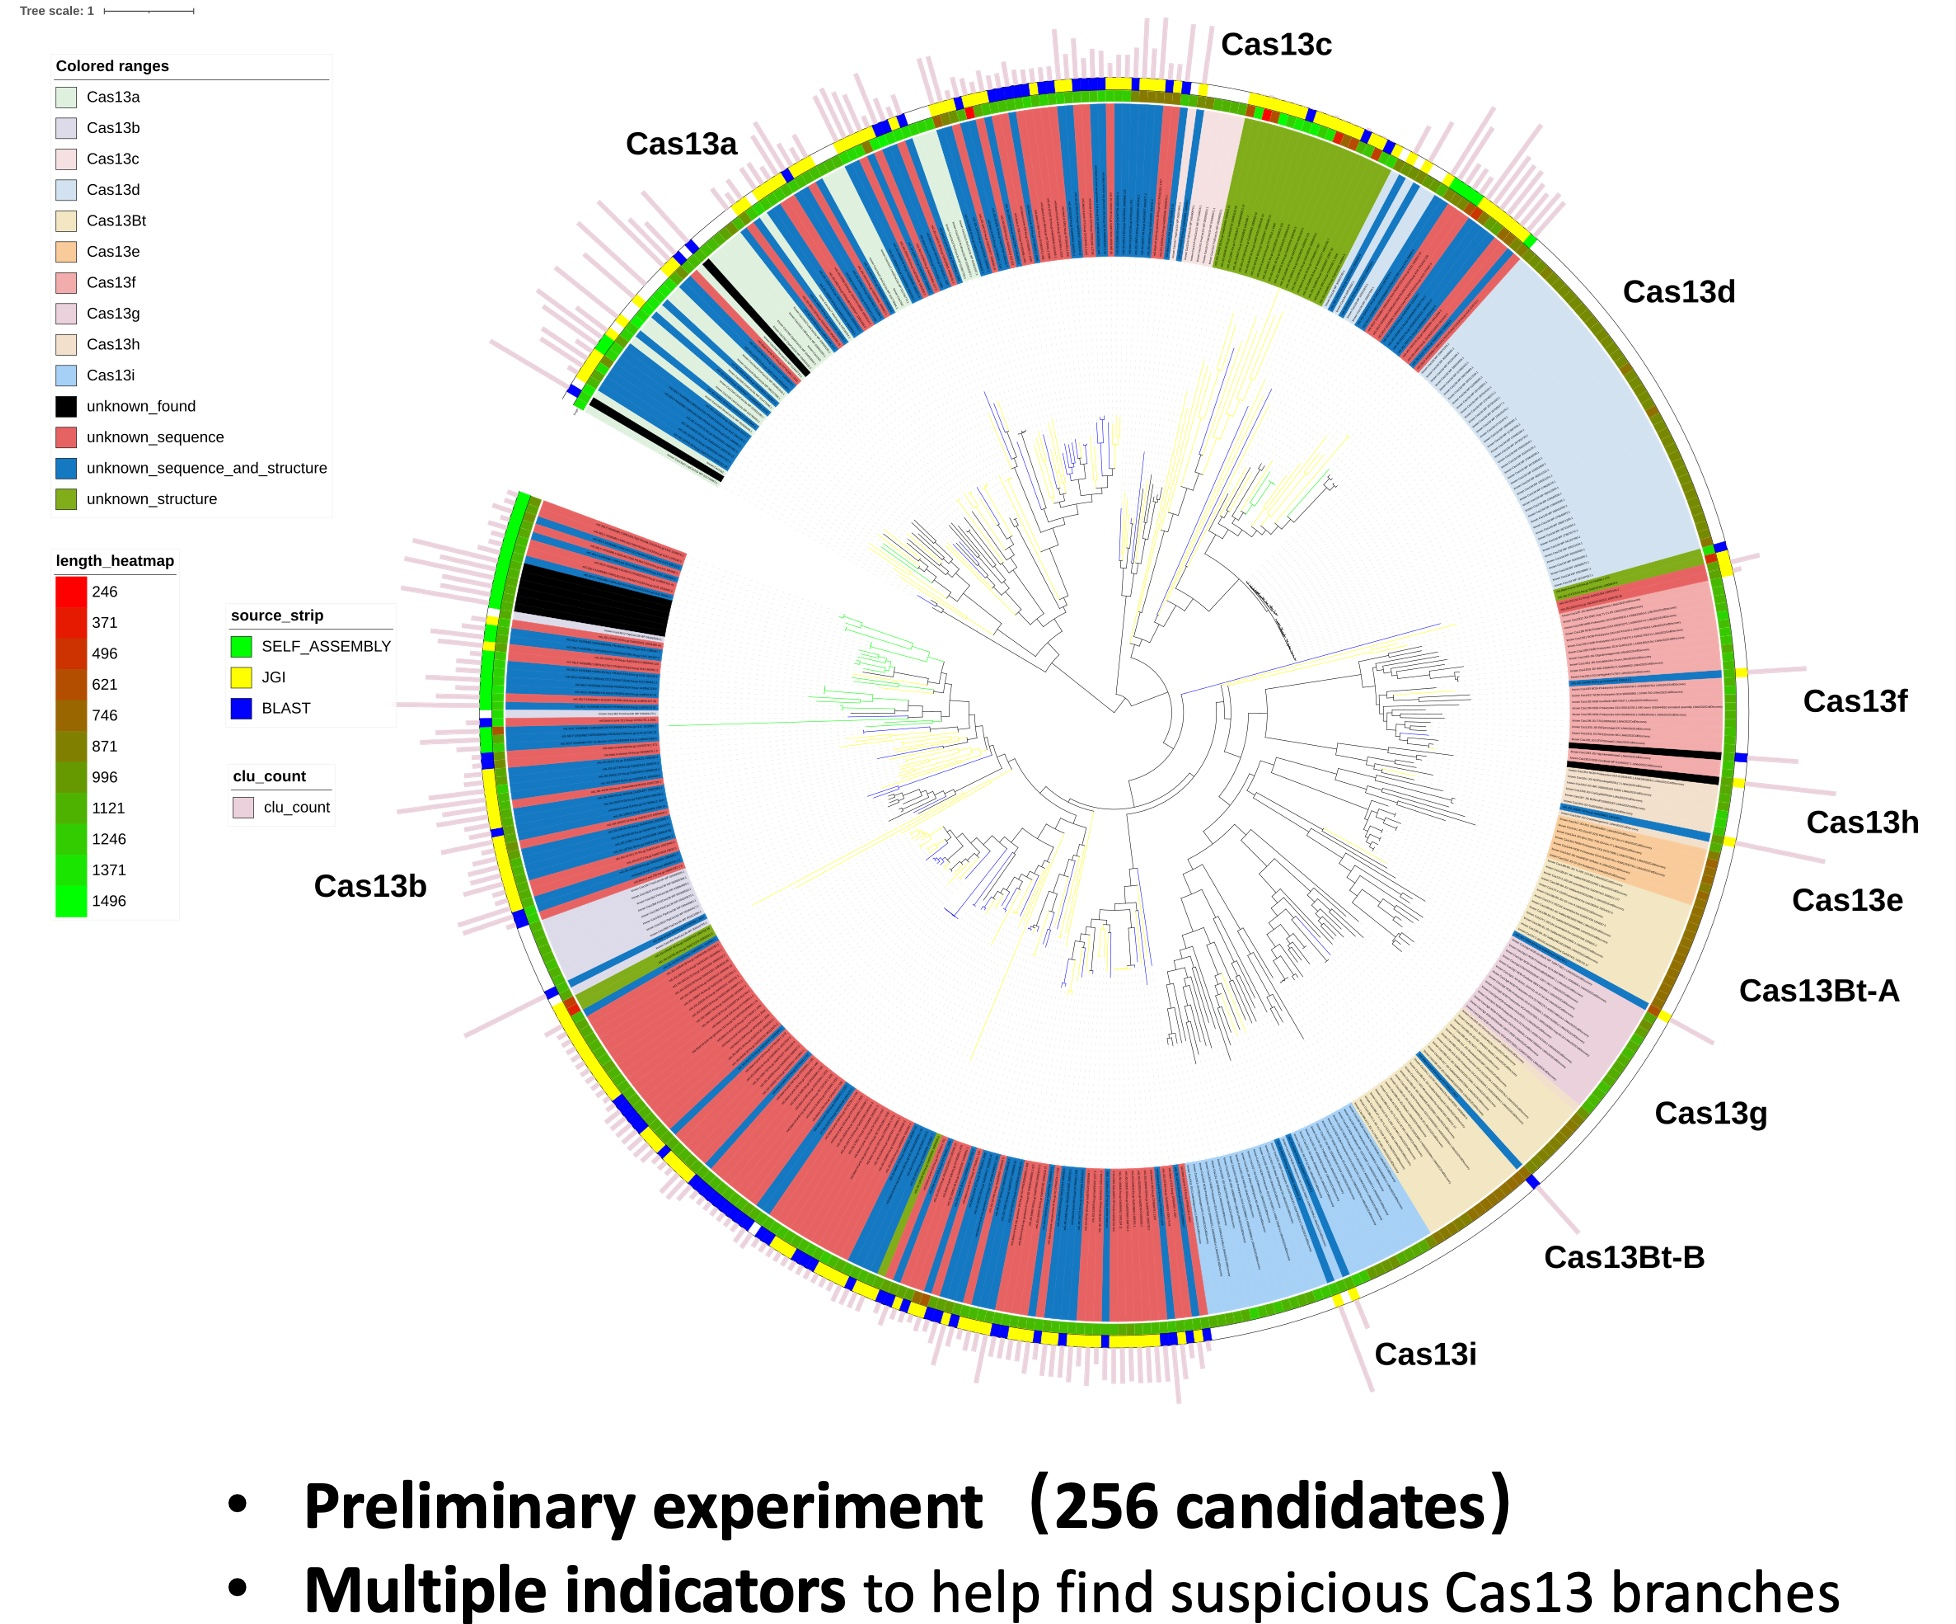
\includegraphics[width=1\textwidth]{figs/Cas13_structure_tree.jpg} 
	\caption{\textbf{Cluster tree of structural similarity}.}
	\label{fig:Cas13_structure_tree}
\end{figure}


%%%%%%%%%%%%%%%% REFERENCES %%%%%%%%%%%%%%%

\clearpage % Clear all remaining figures and tables then start a new page

% The list of references goes after the main text and before the acknowledgements
% When preparing an initial submission, we recommend you use BibTeX, like this:
%
\bibliography{refs} % for a file named science_template.bib
\bibliographystyle{sciencemag}

\end{document}
% End of science_template.tex



